\documentclass{../../../oss-classkick}

\begin{document}
\genheader

\gentitle{1}{HARMONIC MOTION}

\genmultidirections

\gengravity

\raggedcolumns
\begin{multicols}{2}
  \begin{enumerate}[leftmargin=18pt]

  \item A 0.40-kg mass hangs on a spring with a spring constant of 12 N/m.
    The system oscillates with a constant amplitude of 12 cm. What is the
    maximum acceleration of the system?
    \begin{enumerate}[nosep,leftmargin=18pt,label=(\Alph*)]
    \item\SI{.62}{\metre\per\second\squared}
    \item\SI{1.4}{\metre\per\second\squared}
    \item\SI{1.6}{\metre\per\second\squared}
    \item\SI{3.6}{\metre\per\second\squared}
    \item\SI{9.8}{\metre\per\second\squared}
    \end{enumerate}

  \item A mass is attached to a spring and allowed to oscillate vertically.
    Which of the following would NOT change the period of the oscillation?
    \begin{enumerate}[nosep,leftmargin=18pt,label=(\Alph*)]
    \item Double the mass and double the spring constant
    \item Double the amplitude of vibration and double the mass
    \item Double the gravitational field strength and double the mass
    \item Double the gravitational field strength and double the spring constant
    \item Double the gravitational field strength and quadruple the mass
    \end{enumerate}
    \vspace{.7in}
    
  \item The Moon is approximately \SI{384000}{\kilo\metre} from the Earth. The
    Moon revolves around the Earth once every 27.3 days. What is the frequency
    of the Moon's motion?
    \begin{enumerate}[nosep,leftmargin=18pt,label=(\Alph*)]
    \item \SI{14100}{\kilo\metre} each day
    \item 0.0366 revolution each day
    \item 27.3 revolution each day
    \item 655 hours for each revolution
    \item 27.3 days for each revolution
    \end{enumerate}
    \vspace{.7in}
    
  \item A mass is suspended from a spring and allowed to oscillate freely. When
    the amplitude of vibration is doubled, what happens to frequency of
    vibration?
    \begin{enumerate}[nosep,leftmargin=18pt,label=(\Alph*)]
    \item It quadruples.
    \item It doubles.
    \item It stays the same.
    \item It reduces to one-half of what it was.
    \item It reduces to one-fourth of what it was.
    \end{enumerate}
    \vspace{.7in}
    
  \item A bell is rung when the dangling clapper within it makes contact with
    the bell. A poorly designed bell has a clapper that swings with the same
    period as the bell. How can this design be improved?
    \begin{enumerate}[nosep,leftmargin=18pt,label=(\Alph*)]
    \item Use a clapper with a smaller mass on the end so it is out of period
      with the bell.
    \item Use a clapper with a bigger mass on the end so it is out of period
      with the bell.
    \item Force the bell to swing with greater amplitude.
    \item Use a longer clapper so it is out of period with the bell.
    \item Increase the mass of the bell so it makes better contact with the
      clapper.
    \end{enumerate}
    \columnbreak
    
  \item Which choice below best explains why a pendulum does not oscillate
    in zero gravity?
    \begin{enumerate}[nosep,leftmargin=18pt,label=(\Alph*)]
    \item The pendulum has no mass in zero gravity.
    \item A pendulum requires gravity to create the restoring force.
    \item The pendulum is in orbit and considered weightless.
    \item The pendulum would be too far from the Earth to work properly.
    \item The pendulum must have an oscillating tension in the string to
      function properly.
    \end{enumerate}
    \vspace{.7in}
    
  \item A refrigerator compressor that weighs 8 kg is fixed to three separate
    springs on the refrigerator frame. Each has a spring constant of
    \SI{0.01}{\newton\per\metre}. What is the natural frequency of the system?
    \begin{enumerate}[nosep,leftmargin=18pt,label=(\Alph*)]
    \item 0.01 cycle/s
    \item 0.03 cycle/s
    \item 0.8 cycle/s
    \item 103 cycles/s
    \item 0.003 cycle/s
    \end{enumerate}
    \vspace{.7in}
    
  \item A pendulum on the surface of the Moon has a period of 1.0 s. If the
    length of the pendulum is quadrupled, what is the value of the new
    period?
    \begin{enumerate}[nosep,leftmargin=18pt,label=(\Alph*)]
    \item 0.25 s
    \item 0.50 s
    \item 1.0 s
    \item 2.0 s
    \item 4.0 s
    \end{enumerate}
    
  \item A 2.0-m pendulum on a particular planet has a period of 4.6 s. What is
    the gravitational field strength on that planet?
    \begin{enumerate}[nosep,leftmargin=18pt,label=(\Alph*)]
    \item\SI{1.6}{\newton\per\kilo\gram}
    \item\SI{3.7}{\newton\per\kilo\gram}
    \item\SI{4.9}{\newton\per\kilo\gram}
    \item\SI{9.8}{\newton\per\kilo\gram}
    \item\SI{25}{\newton\per\kilo\gram}
    \end{enumerate}

  \item The displacement (in centimeters) of the vibrating cone of a large
    loudspeaker is represented by the equation $\Delta x=2.0\cos(150t)$, where
    $t$ is the time in seconds. What distance does the tip of the cone move in
    half a period?
    \begin{enumerate}[nosep,leftmargin=18pt,label=(\Alph*)]
    \item 0.007 cm
    \item 1.0 cm
    \item 2.0 cm
    \item 4.0 cm
    \item 150 cm
    \end{enumerate}

  \item Which choice below best explains why a pendulum does not oscillate
    in zero gravity?
    \begin{enumerate}[nosep,leftmargin=18pt,label=(\Alph*)]
    \item The pendulum has no mass in zero gravity.
    \item A pendulum requires gravity to create the restoring force.
    \item The pendulum is in orbit and considered weightless.
    \item The pendulum would be too far from the Earth to work properly.
    \item The pendulum must have an oscillating tension in the string to
      function properly.
    \end{enumerate}
    \columnbreak
    
  \item Some large oil tankers have an antiroll water tank inside the hull that
    matches the resonant frequency of the ship’s hull. When ocean waves hit the
    ship at the resonant frequency, how does the water tank prevent the ship
    from capsizing in the waves?
    \begin{enumerate}[nosep,leftmargin=18pt,label=(\Alph*)]
    \item The energy of the waves is used by the water in the tank.
    \item The waves enter the tank and are dampened.
    \item The water tank is \ang{180} out of phase with the ship's hull.
    \item The water tank is \ang{90} out of phase with the ship's hull.
    \item The water in the tank is in phase with the ship's hull.
    \end{enumerate}
    \vspace{.7in}
    
  \item The graph below shows the displacement versus time for an object. Which
    equation best describes its displacement in meters?
    \cpic{.45}{d-t}
    \begin{enumerate}[nosep,leftmargin=18pt,label=(\Alph*)]
    \item $\Delta x=20\cos(0.5t)$
    \item $\Delta x=10\cos(2t)$
    \item $\Delta x=10\cos(\pi t)$
    \item $\Delta x=20\cos(2t)$
    \item $\Delta x=20\sin(\pi t)$
    \end{enumerate}
    \vspace{.7in}
    
  \item The Moon has a gravitational field strength that is approximately
    one-sixth of the field on the Earth. What is the ratio between the period
    of a pendulum on the Moon and the period of an identical pendulum on the
    Earth?
    \begin{enumerate}[nosep,leftmargin=18pt,label=(\Alph*)]
    \item 6
    \item $\sqrt{6}$
    \item $\displaystyle\frac16$
    \item $\displaystyle\frac1{\sqrt6}$
    \item 1
    \end{enumerate}

  \item Which of the following best represent periodic motion?
    \begin{enumerate}[nosep,leftmargin=18pt,label=(\Alph*)]
    \item A skydiver who has reached terminal velocity
    \item The Moon in orbit about the Earth
    \item A car driving to each state in the United States
    \item A cart pushed up a frictionless incline plane
      %\item A pendulum swinging over a 30-min time span.
    \item A rubber ball bouncing on the floor over 30 seconds.
    \end{enumerate}
    \vspace{.7in}
    
  \item  Which of the following significantly affect the period of a simple
    pendulum?
    \begin{enumerate}[nosep,leftmargin=18pt,label=(\Alph*)]
    \item The length of the pendulum
    \item The mass of the pendulum bob
    \item The amplitude of swing
      %\item The gravitational field strength
    \item The shape of the mass
    \item The thickness of the string
    \end{enumerate}
    \columnbreak    

  \item A particle oscillates with simple harmonic motion with no damping.
    Which one of the following statements about the acceleration of the
    oscillating particle is true?
    \begin{enumerate}[nosep,leftmargin=18pt,label=(\Alph*)]
    \item It has a value of \SI{9.8}{\metre\per\second\squared} when the
      oscillation is vertical.
    \item It is zero when the speed is the minimum.
    \item It is proportional to the frequency.
    \item It is zero throughout the oscillation.
    \item It is zero when the speed is the maximum.
    \end{enumerate}
  \end{enumerate}
  
  \textbf{Questions \ref{one}--\ref{four}} are based on the figure below of a
  mass-spring system. Assume the mass is pulled back to position +A and
  released, and it slides back and forth without friction.
  \begin{center}
    \pic{.3}{springs}
  \end{center}
  \begin{enumerate}[leftmargin=18pt,resume]
  \item When the mass reaches position $-A$, what can be said about its speed?
    \label{one}
    \begin{enumerate}[nosep,leftmargin=18pt,label=(\Alph*)]
    \item It is a minimum.
    \item It is a maximum.
    \item It is zero.
    \item It is decreasing.
    \item It is increasing.
    \end{enumerate}
    \vspace{.7in}
    
  \item When the mass reaches position 0, what can be said about its speed?
    \begin{enumerate}[nosep,leftmargin=18pt,label=(\Alph*)]
    \item It is a minimum.
    \item It is a maximum.
    \item It is zero.
    \item It is decreasing.
    \item It is increasing.
    \end{enumerate}
    \vspace{.7in}
    
  \item At what position does the mass have the greatest acceleration?
    \begin{enumerate}[nosep,leftmargin=18pt,label=(\Alph*)]
    \item $-A$
    \item $-A/2$
    \item 0
    \item $+A/2$
    \item $+A$
    \end{enumerate}
    
  \item The mass is released from the $-A$ position at time $t=0$, and it
    oscillates with period $T$, measured in seconds. Which equation best
    represents the displacement?
    \label{four}
    \begin{enumerate}[nosep,leftmargin=18pt,label=(\Alph*)]
    \item $\displaystyle \Delta x = -A\cos\left(\frac{T}{2\pi}t\right)$
    \item $\displaystyle \Delta x = -(A/2)\cos(2\pi T t)$
    \item $\displaystyle \Delta x = -A\cos\left(\frac{2\pi}{T}t\right)$
    \item $\displaystyle \Delta x = (A/2)\cos(T t)$
    \item $\displaystyle \Delta x = A\cos\left(\frac{2\pi}{T}t\right)$
    \end{enumerate}
  \end{enumerate}
\end{multicols}
\newpage

\genfreetitle{1}{SIMPLE HARMONIC MOTION}{4}

\genfreedirections

% QUESTION IS TAKEN FROM 2018 AP PHYSICS 1 FREE-RESPONSE QUESTION #5
\cpic{.5}{blocks}
\begin{enumerate}
\item %(7 points, suggested time 13 minutes)
  Block $P$ of mass $m$ is on a horizontal, frictionless surface and is
  attached to a spring with spring constant $k$. The block is oscillating with
  period $T_P$ and amplitude $A_P$ about the spring's equilibrium position
  $x_0$. A second block $Q$ of mass $2m$ is then dropped from rest and lands on
  block $P$ at the instant it passes through the equilibrium position, as shown
  above. Block $Q$ immediately sticks to the top of block $P$, and the
  two-block system oscillates with period $T_{PQ}$ and amplitude $A_{PQ}$.
  \begin{enumerate}
  \item Determine the numerical value of the ratio $T_{PQ}/T_P$.
  \item How does the amplitude of oscillation $A_{PQ}$ of the two-block system
    compare with the original amplitude $A_P$ of block $P$ alone?

    \vspace{.1in}
    \underline{\hspace{.3in}} $A_{PQ}<A_{P}$\hspace{.25in}
    \underline{\hspace{.3in}} $A_{PQ}=A_{P}$\hspace{.25in}
    \underline{\hspace{.3in}} $A_{PQ}>A_{P}$

    \vspace{.2in}In a clear, coherent paragraph-length response that may also
    contain diagrams and/or equations, explain your reasoning.
  \end{enumerate}
  \newpage
  
\item In heavy seas, the bow of a battle ship undergoes a simple harmonic
  vertical pitching motion with a period of \SI{8.}{\second} and an amplitude
  of \SI{2.}{\metre}.
  \begin{enumerate}
  \item What is the maximum vertical velocity of the battle ship's bow?
  \item What is its maximum acceleration?
  \item An \SI{80}{\kilo\gram} sailor is standing on the scale in the bunk room
    in the bow. What are the maximum and minimum reading on the scale in
    newtons?
  \end{enumerate}
  \newpage
  
\item Show that for the situations in the figures below, the object of mass
  $m$ oscillates with a frequency of
  $\displaystyle\omega=\sqrt{\frac{k_\text{eff}}{m}}$ where $k_\text{eff}$ is
  given by (a) $k_\text{eff}=k_1+k_2$ and (b)
  $\displaystyle\frac1{k_\text{eff}}=\frac1{k_1}+\frac1{k_2}$. Hint:
  find the net force on the mass and write $F=-k_\text{eff}x$. Note that in
  (b), the springs stretch by different amounts, the sum of which is $x$.
  
  (a)\hspace{5pt}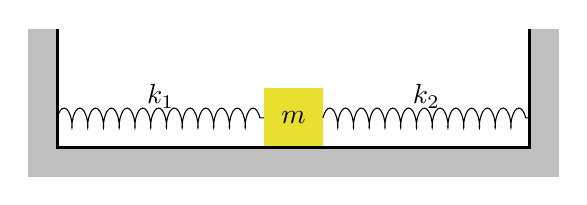
\begin{tikzpicture}[scale=.5]
    \fill[gray!50](0,0) rectangle(12,-.75);
    \fill[gray!50](-.75,-.75) rectangle(0,3);
    \fill[gray!50](12,-.75) rectangle(12.75,3);
    \fill[yellow!80!gray](5.25,0) rectangle(6.75,1.5) node[midway,black]{$m$};
    \draw[decoration={aspect=0.3,segment length=2mm, amplitude=1.25mm, coil},
      decorate] (0,.75)--(5.25,.75) node[midway,above]{$k_1$};
    \draw[decoration={aspect=0.3,segment length=2mm, amplitude=1.25mm, coil},
      decorate] (6.75,.75)--(12,.75) node[midway,above]{$k_2$};
    \draw[very thick](0,3)--(0,0)--(12,0)--(12,3);
  \end{tikzpicture}
  
  (b)\hspace{5pt}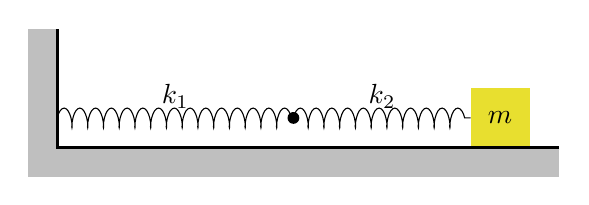
\begin{tikzpicture}[scale=.5]
    \fill[gray!50](0,0) rectangle(12.75,-.75);
    \fill[gray!50](-.75,-.75) rectangle(0,3);
    \fill[yellow!80!gray](10.5,0) rectangle(12,1.5) node[midway,black]{$m$};
    \draw[decoration={aspect=0.3,segment length=2mm, amplitude=1.25mm, coil},
      decorate] (0,.75)--(6,.75) node[midway,above]{$k_1$};
    \draw[decoration={aspect=0.3,segment length=2mm, amplitude=1.25mm, coil},
      decorate] (6,.75)--(10.5,.75) node[midway,above]{$k_2$};
    \fill[black](6,.75) circle(.15);
    \draw[very thick](0,3)--(0,0)--(12.75,0);
  \end{tikzpicture}
  \newpage
  
\item A simple pendulum of length $L$ is released from rest from an angle of
  $\theta_0$.
  \begin{enumerate}
  \item Assuming the motion of the pendulum to be simple harmonic motion, find
    its speed as it passes through $\theta=0$.
  \item Using the conservation of energy, find this speed exactly.
  \item Show that your results for (a) and (b) are the same when $\theta_0$ is
    small.
  \item Find the difference in your results for $\theta_0=\SI{.20}{rad}$ and
    $L=\SI{1}{\metre}$.
  \end{enumerate}
\end{enumerate}
\end{document}
